\paragraph{Implementation of Prim's algorithm in $O\left(n^{2}\right)$}

Prim's algorithm is based on graph traversals (visiting every vertex in the graph), which are inherently difficult to parallelize. It also has an irregular memory access pattern. In CPUs, this limits the use of the cache and leads to an overall performance penalty. The prim's algorithm is highly dependent on the organization of memory storage and memory access patterns.\cite{10.1007/978-3-642-38853-8_14}

\highspace
The following data structure we propose guarantees a complexity of $O\left(n^{2}\right)$.
\begin{itemize}
    \item $k$ is the number of edges selected so far;

    \item $S$ is the subset $S \subseteq N$ of nodes incident to the selected edges (same as explained in the \ref{paragraph: Prim's algorithm} section, page \pageref{paragraph: Prim's algorithm});
    
    \item $T$ is the subset $T \subseteq E$ of selected edges (same as explained in the \ref{paragraph: Prim's algorithm} section, page \pageref{paragraph: Prim's algorithm});
    
    \item $C_{j}$ is a vector which has a value equal to:
    \begin{equation*}
        C_{j} = \begin{cases}
            \min\left\{c_{ij} \: : \: i \in S\right\} & j \notin S \\
            \infty & \text{otherwise}
        \end{cases}
    \end{equation*}
    At the beginning of the algorithm it is clearly composed of infinite values if the edge $i$ to $j$ doesn't exist, otherwise the weight of the edge. In the core of the algorithm, each position is updated with the minimum weighted edge value.
    
    \item $\text{closest}_{j}$ is a vector which has a value equal to:
    \begin{equation*}
        \text{closest}_{j} = \begin{cases}
            \mathrm{argmin}\left\{c_{ij} \: : \: i \in S\right\} & j \notin S \\
            \text{predecessor of }j\text{ in the minimum spanning tree} & j \in S
        \end{cases}
    \end{equation*}
    The node closest to the edge has less weight, otherwise if we look at the node $j$ in the set $S$, the predecessor of that node in the minimum spanning tree. A trivial example:
    \begin{figure}[!htp]
        \centering
        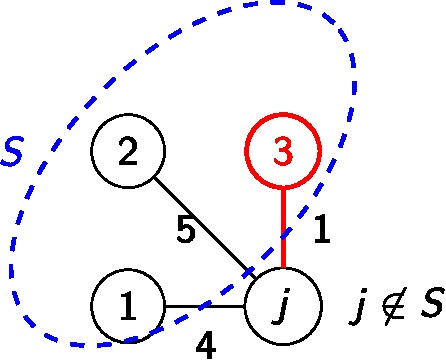
\includegraphics[width=.3\textwidth]{img/prims-alg-7.pdf}
    \end{figure}
    
    With $\mathrm{closest}_{j} = 3$ and $c_{\mathrm{closest}_{j}},j = 1$.
\end{itemize}
Let's take an example to clear up any doubts.

\begin{examplebox}[: Prim's algorithm $O\left(n^{2}\right)$]
    Suppose we have the following graph:
    \begin{center}
        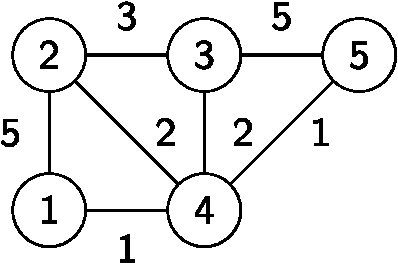
\includegraphics[width=.3\textwidth]{img/prims-alg-1.pdf}
    \end{center}

    \begin{enumerate}
        \item At the beginning we choose an arbitrary node $u$ that is in the set $N$, for example $3$. We set the set of transitions $T$ to the empty set, the set of evaluated nodes $S$ to the selected node $u$, in our case the value 3, and finally the two vectors. The vector $C_{j}$ is filled of infinite values if the edge $u$ to $j$ doesn't exist, otherwise the weight of the edge, and the vector $\text{closest}_{j}$ is filled with the selected starting node, in our case 3.
        \begin{itemize}
            \item $T = \emptyset$
            \item $S = \left\{u\right\} = \left\{3\right\}$
            \item $C_{j} = \left[+\infty, 3, -, 2, 5\right]$
            \item $\text{closest}_{j} = \left[3, 3, -, 3, 3\right]$
        \end{itemize}
        Some observations:
        \begin{itemize}
            \item The symbol $-$ is the \href{https://en.wikipedia.org/wiki/Don%27t-care_term}{don't care term used in digital logic}.
            \item The position of each value respects the j-index. For example, the node 3 in the vectors $C_{j}$ and $\text{closest}_{j}$ is placed at position number 3. The value is don't care ($-$) because it is the starting point. The other values depend on the graph. Node 1 has no direct edge to node 3, so it has an infty value; node 2 has a direct edge with weight 3; node 3 doesn't care because it's the starting point; and so on.
        \end{itemize}
        \begin{center}
            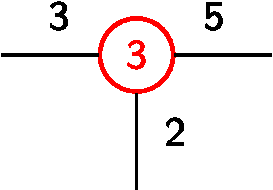
\includegraphics[width=.2\textwidth]{img/prims-alg-2-imp.pdf}
        \end{center}

        \item The minimum value in $C_{j}$ is 2 and since it is in the 4th position, node 4 is selected.
        \begin{itemize}
            \item $T = \left\{\left\{3,4\right\}\right\}$
            \item $S = \left\{3, 4\right\}$
            \item $C_{j} = \left[\mathbf{1}, \mathbf{2}, -, 2, \mathbf{1}\right]$
            \item $\text{closest}_{j} = \left[\mathbf{4}, \mathbf{4}, -, 3, \mathbf{4}\right]$
        \end{itemize}
        The values updated are the first, second and fifth positions, as nodes three and four are in the $S$ set.
        \begin{center}
            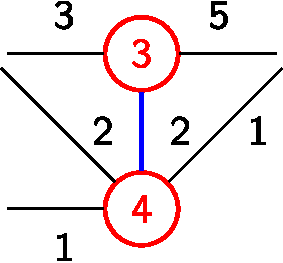
\includegraphics[width=.2\textwidth]{img/prims-alg-3-imp.pdf}
        \end{center}

        \item The minimum value in $C_{j}$ is the first position. But the fifth position is also the minimum. We choose the first value because the vector is analyzed sequentially (first to last).
        \begin{itemize}
            \item $T = \left\{\left\{3,4\right\}, \left\{1,4\right\}\right\}$
            \item $S = \left\{1, 3, 4\right\}$
            \item $C_{j} = \left[1, \mathbf{2}, -, 2, \mathbf{1}\right]$
            \item $\text{closest}_{j} = \left[4, \mathbf{4}, -, 3, \mathbf{4}\right]$
        \end{itemize}
        \begin{center}
            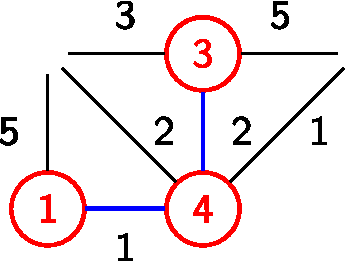
\includegraphics[width=.25\textwidth]{img/prims-alg-4-imp.pdf}
        \end{center}

        \item The minimum value in $C_{j}$ is quite trivial, between 2 and 1. We choose the value 1 and the node $4$ is the closest.
        \begin{itemize}
            \item $T = \left\{\left\{3,4\right\}, \left\{1,4\right\}, \left\{4,5\right\}\right\}$
            \item $S = \left\{1, 3, 4, 5\right\}$
            \item $C_{j} = \left[1, \mathbf{2}, -, 2, 1\right]$
            \item $\text{closest}_{j} = \left[4, \mathbf{4}, -, 3, 4\right]$
        \end{itemize}
        \begin{center}
            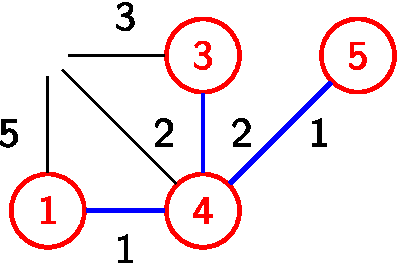
\includegraphics[width=.3\textwidth]{img/prims-alg-5-imp.pdf}
        \end{center}

        \item Finally, node 2 with edge weight 2 is selected.
        \begin{itemize}
            \item $T = \left\{\left\{3,4\right\}, \left\{1,4\right\}, \left\{4,5\right\}, \left\{2,4\right\}\right\}$
            \item $S = \left\{1, 2, 3, 4, 5\right\} = N$
            \item $C_{j} = \left[1, 2, -, 2, 1\right]$
            \item $\text{closest}_{j} = \left[4, 4, -, 3, 4\right]$
        \end{itemize}
        \begin{center}
            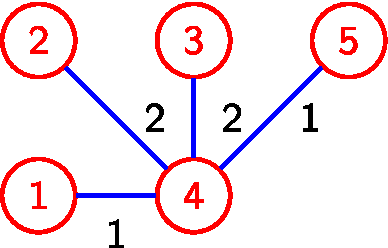
\includegraphics[width=.3\textwidth]{img/prims-alg-6-imp.pdf}
        \end{center}
    \end{enumerate}
\end{examplebox}

\noindent
\begin{flushleft}
    \textcolor{Green3}{\faIcon{question-circle} \textbf{Ok, but how do we get the spanning tree from the nearest vector?}}
\end{flushleft}
The minimum spanning tree found by Prim's algorithm consists of the $n-1$ edges:
\begin{equation*}
    \left\{\text{closest}_{j}, j\right\} \hspace{2em} \text{with } j = 1,2,\dots,n
\end{equation*}
For example, from the previous example, let the \emph{closest} vector:
\begin{equation*}
    \text{closest}_{j} = \left[4,4,-,3,4\right]
\end{equation*}
A minimum cost spanning tree consists of the edges:
\begin{equation*}
    \left\{4,1\right\}, \left\{4,2\right\}, \cancel{\left\{-,-\right\}}, \left\{3,4\right\}, \left\{4,4\right\}
\end{equation*}
\begin{lstlisting}[language=pseudo-code, caption={Minimum spanning tree (MST) problem: Prim's $O\left(n^{2}\right)$}]
S $\leftarrow$ $\{$u$\}$; $\label{prims-imp: s-definition}$
T $\leftarrow$ $\emptyset$; $\label{prims-imp: t-definition}$
for $j \in N \setminus S$ do: $\label{prims-imp: for j in N setminus S}$
    $C_{j} \leftarrow c_{uj}$; // or $+\infty$ if $\left\{u,j\right\} \notin E$
    $\text{closest}_{j} \leftarrow u$; $\label{prims-imp: end for}$
for $k = 1, \dots, n-1$ do: $\label{prims-imp: for k from 1 to n-1}$
    // select min edge in $\delta(S)$
    min $\leftarrow +\infty$; $\label{prims-imp: start select minimum edge}$
    for $j = 1, \dots, n$ do: $\label{prims-imp: third for}$
        if $j \notin S$ and $C_{j} <$ min:
            min $\leftarrow C_{j}$;
            v $\leftarrow$ j; $\label{prims-imp: end select minimum edge}$
    // extend S and T
    S $\leftarrow$ S $\cup \left\{v\right\}$; $\label{prims-imp: start extend S and T}$
    T $\leftarrow$ T $\cup \left\{\left\{\text{closest}_{v}, v\right\}\right\}$; $\label{prims-imp: end extend S and T}$
    // update $C_{j}$ and $\text{closest}_{j}$, $\forall j \notin S$
    for $j = 1, \dots, n$ do: $\label{prims-imp: for j from 1 to n}$
        if $j \notin S$ and $c_{vj} < C_{j}$:
            $C_{j} \leftarrow c_{vj}$;
            $\text{closest}_{j} \leftarrow v$; $\label{prims-imp: end for j from 1 to n}$
\end{lstlisting}
\begin{itemize}
    \item[Rows \ref{prims-imp: s-definition}-\ref{prims-imp: t-definition}.] Declare the general sets $S$ and $T$. The first is filled with the starting node $u$ and the second is empty, because the core of the algorithm has not yet started.

    \item[Rows \ref{prims-imp: for j in N setminus S}-\ref{prims-imp: end for}.] The first for statement is used to initialize the two vectors $C_{j}$ and $\text{closest}_{j}$. It inserts the edge weight into $C_{j}$ if there is a direct edge from $u$ to $j$, otherwise infinity is used. Meanwhile, the \emph{closest} vector consists only of the starting node $u$ at the beginning of the algorithm.

    \item[Row \ref{prims-imp: for k from 1 to n-1}.] The second for statement is the core of the algorithm. Here the index goes from one to the number of nodes minus one.
    
    \item[Rows \ref{prims-imp: start select minimum edge}-\ref{prims-imp: end select minimum edge}.] This piece of code is used to select the minimum edge available in the $C_{j}$ vector. It starts by setting the \texttt{min} variable to infinity, to ensure that a value is selected. Therefore, the for statement iterates over each node; at each iteration, if the selected node is not in the $S$ set (so it has not already been evaluated) and the value at the corresponding position in the vector $C_{j}$ is less than minimum, then assign to the minimum the value of the vector $C_{j}$ at position $j$ and to $v$ the index $j$.

    \item[Rows \ref{prims-imp: start extend S and T}-\ref{prims-imp: end extend S and T}.] Now it updates the variable $S$ with the node $v$ and the transitions set with the tuple (value at the corresponding position in the vector $\text{closest}_{v}$, node $v$).

    \item[Rows \ref{prims-imp: for j from 1 to n}-\ref{prims-imp: end for j from 1 to n}.] There is another for statement similar to the previous one, because here it needs to update the vectors $C_{j}$ and $\text{closest}_{j}$ with the new values. The for iterates over every node of the graph. So at each iteration it checks that the selected vertex is not in the $S$-set (not already evaluated) and that the weight of the edge from vertex $v$ to $j$ (if it exists, otherwise infinity) is less than the value $C_{j}$. If the double condition is true, it updates the two vectors at position $j$.
\end{itemize}
The overall complexity is given by:
\begin{itemize}
    \item The number of iterations of the first for at row \ref{prims-imp: for j in N setminus S}, which is: $\left(n-1\right)$

    \item Plus the number of iterations of the second for at row \ref{prims-imp: for k from 1 to n-1}, which is: $\left(n-1\right)$
    
    \item Times the number of iterations of the third and fourth for at lines \ref{prims-imp: third for} and \ref{prims-imp: for j from 1 to n}, which is: $\left(n-1+n-1\right)$
\end{itemize}
The result is $O\left(n^{2}\right)$. For sparse graphs, a more sophisticated data structure leads to an $O\left(m \log n\right)$ complexity.